Ahora, dado que ya disponemos de todas las partes del sistema convenientemente dispuestas y calibradas, procedemos a realizar una primera medida.

Hay que tener en cuenta que en estas primeras medidas no necesitamos un sistema de control de temperatura ya que vamos a utilizar PMT y estos no son tan sensibles a la temperatura como los SiPM. Únicamente deberemos ser capaces de evitar oscilaciones grandes de temperatura ($\Delta T=15-20ºC$), los cuales si afectan de forma apreciable a la ganancia del PMT. Esto lo podemos conseguir manteniendo el aire acondicionado de la sala experimental encendido y programado a una misma temperatura durante las medidas. 

Sin embargo, cuando vayamos a realizar las medidas del prototipo con SiPMs, si necesitaremos este control exaustivo de la temperatura ya que, como se vió en la sección de calibrado del SiPM, \ref{sec:Temperatura}, existe una dependencia muy marcada. Se necesitará adquirir un sistema de control de temperatura o, en su defecto, como construir y calibrar uno nosotros mismos.

La primera medida se realizará sin coincidencia, pasando directamente la señal 1 al MCA. El MCA nos permite obtener un histograma energético.

Se obtendrá un primer histograma del prototipo con agua hiperpura y sin tritio. Dado que el agua hiperpura idealmente no añade ningun tipo de contribución al histograma llamaremos a esta medida señal de fondo. 

Seguidamente se rellenará el prototipo con agua tritiada y se obtendrá un segundo histograma. En esta segunda medida se pude observar en el display del MCA que el número de cuentas medidas por segundo era mayor que el la medida del fondo. Esto es un indicativo de que estamos detectando tritio. 

Finalmente se normalizan cada uno de los histogramas al tiempo correspondiente a su medida para obtener histogramas de actividad en lugar de un histograma de sucesos. Los tiempos asociados al histograma del tritio y del fondo son $T_S=154143~\second$  y $T_B=246987~\second$, respectivamente, medidas largas para tener suficiente estadística. El resultado puede verse en la figura 26 izquierda. Además se ha añadido una segunda imagen, figura 26 derecha, en la cual se ha realizado representado la señal con tritio a la cual se le ha extraido la señal de fondo, es decir, en esta segunda imagen encontramos la señal debida únicamente al tritio.

\begin{figure}[hbtp]
\centering
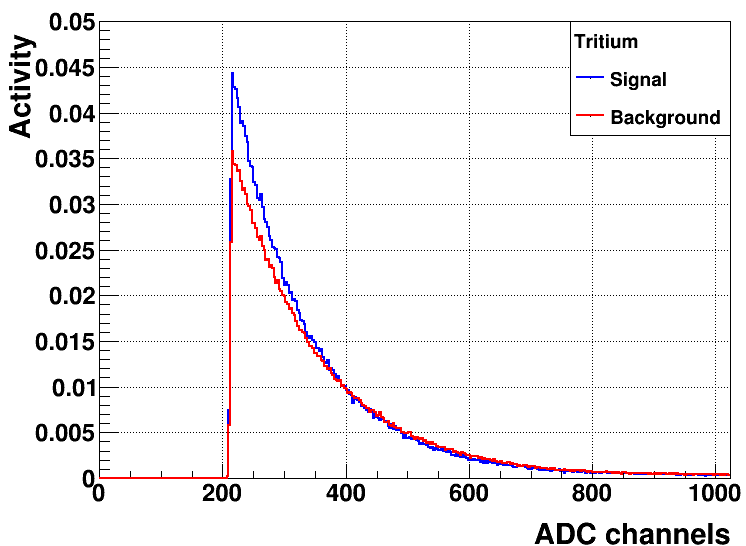
\includegraphics[scale=0.4]{Tritium3-fcpst2.png}
\caption{Histograma energético de la señal del prototipo de tritios y del fondo superpuestos.\label{tritiofondo}}
\end{figure}

En esta figura podemos observar que estamos detectando un pico de señal de aproximadamente $0.045~\becquerel$ y una señal debida únicamente a tritio de aproximadamente $0.01~\becquerel$. POdemos apreciar la existencia de una zona entre los canales 450 y 700 donde el fondo supera a la señal. Habrá que indagar más en este prototipo para encontrar la explicación de este fenómeno.

Para ver hasta que punto nuestro sistema funciona de forma adecuada podemos realizar un rápido cálculo para ver cual es la actividad detectada que deberíamos esperar. Para ello por un lado calcularemos el volumen efectivo de la fuente y, por otro lado, utilizaremos este volumen para determinar cual es la actividad que deberíamos medir teóricamente en nuestro experimento.

\begin{itemize}
 \item{} Para calcular el volumen efectivo de la fuente tenemos en cuenta que los electrones procedentes de la desintegración del tritio poseen un recorrido libre medio de $5~\mu m$. Por tanto únicamente contribuira de forma apreciable a la señal el agua tritiada que se encuentre formando un cilindro de groson $5~\mu m$ alrededor de cada fibra. Pasamos a calcular este volumen. Para ello calcularemos el volumen total y, a esta cantidad, le extraeremos el volumen ocupado por la fibra.

El volumen de la fibrá es el volumen correspondiente a un cilindro de radio $0.5~\mm$ (radio de la fibra) y una longitud efectiva de $20~\cm$, donde se ha tenido en cuenta que, aunque la longitud real de la fibra son $25~\cm$, esta contiene en los extremos del bunch unos aros metálicos y, además, parte de esta fibra sobresale del prototipo para acoplar a los PMTs. Por extensión, esta sección de la fibra, aproximadamente $2,5~\cm$ a cada extremo,  no contribuyen a la señal de detección del tritio. Con todo esto el volumen ocupado por la fibra será $V_{fibra}=1.5708 \cdotp 10^{-4}$ litros.

Análogamente calculamos el volumen ocupado por la fuente más la fibra, que corresponderá a un cilindro de radio $0.5~\mm+5\mu m$ (radio de la fibra + radio efectivo de la fuente) y la misma longitud que la fibra, es decir, $20~\cm$, ya que en estos extremos se encuentra el final del prototipo. Como resultado el volumen ocupado por la fibra y la parte de la fuente que contribuye a la señal de esta fibrá será $V_{total}=1.6023 \cdotp 10^{-4}$ litros. 

Por tanto el volumen ocupado únicamente por el porcentaje de la fuente que esta interviniendo en la señal de esta fibra será la diferencia entre estos $\V_{fuente}=3.1573 \cdotp 10^{-6}$ litros.
 
Por tanto, teniendo en cuenta que el prototipo únicamente dispone de un bunch formado por 35 fibras centelleadoras el volumen efectivo final del agua tritiado que estamos detectando será el anterior multiplicado por 35, es decir, $1.1050 \cdotp 10^{-4}$ L. 

Hay que tener en cuenta que en esta última multiplicación se ha supuesto que el volumen del agua tritiada asociadas a cada fibra forman un conjunto disjunto y sabemos que esto no es así ya que se producen solapamientos entre ellos. Debido a ello este cálculo será únicamente aproximado.

\item{} Ahora procedemos a calcular la actividad del prototipo conociendo el volumen de agua tritiada que esta aportando a la señal total. Para ello tenemos en cuenta que la disolución posee $2.0169 \pm 0.0017~\gram$ de tritio con una actividad específica de $26.8 \pm 0.6~\mega\becquerel/\gram$ disueltos en medio litro de agua hiperpura (Sec. $\ref{sec:Llenado}$). Con esto podemos calclularnos la actividad total de la disolución, la cual será aproximadamente de $108.11~\mega\becquerel/L$. 

Por tanto, si en medio litro hay aproximadamente $1.0811\cdotp 10^{8}$ desintegraciones por segundo en el volumen calculado anteriormente habrá aproximadamente $2.3893\cdotp 10^{4}$ desintegraciones por segundo.

Finalmente, teniendo en cuenta que la eficiencia de la fibras y de los PMTs son, aproximadamente, 3\% y 30\% respectivamente y suponiendo que la cadena electrónica posee una eficiencia del 100\% llegamos a que la actividad que deberíamos detectar es, aproximadamente $215.03~\becquerel$.

\end{itemize}

Podemos ver que estamos detectando 4 ordenes de magnitud menos de lo que deberíamos. Por un lado esto es debido a imperfecciones del sistema pero la principal fuente de la pérdida de la señal es el hecho de que las fibras empleadas en este prototipo no poseen clad. 

El clad hace que los fotones sean conducidos por el interior de las fibras a partir de reflexiones hasta el contador de fotones, es decir, actua como guia de luz, por tanto, en nuestro prototipo, muchos de los fotones de emisión de las fibras escaparán de estas llegando al agua y, por tanto, producirán pérdida de señal. 

Como resultado únicamente detectaremos el porcentaje asociado al ángulo sólido cubierto por las fibras centelleadoras respecto al total de electrones emitidos por el tritio, cuya emisión supondremos isótropa. Además, del total de fotones reemitidos por las fibras centelleadoras (de nuevo se supone emisión isótropa) ante la detección de este electrón, únicamente detectaremos el porcentaje asociado al ángulo sólido cubierto por la cara final de la fibra centelleadora. También hay que tener en cuenta que el porcentaje de fibra que se encuentra en la parte inferior de la U que conforma el prototipo apenas intervendrá en la señal ya que vemos que prácticamente la totalidad de esta será perdida (su ángulo sólido es cero). 

Podemos realizar una rápida estimación de la magnitud relativa de estos ángulos sólidos para ver su importancia en la pérdida de la señal. Integrando la expresión del ángulo sólido esta toma la siguiente forma: $\Omega=2\pi(1-\cos{\theta})$ donde $\theta$ es el ángulo que subtiene la superficie que queremos calcular$~\cite{unizar}$. Por tanto, dado que la superficie total de emisión será $4\pi$ ($\theta=180º$) el factor de reducción debido al ángulo sólido será $\frac{\Omega}{4\pi}=\frac{1-\cos{\theta}}{2}$. 

Si nos calculamos el ángulo y, por extensión, este factor para el caso del ángulo sólido subtendido por la fibra centelleadora vemos que este ángulo siempre será aproximadamente $90º$ debido al hecho quela fibra centelleadora es mucho mayor que su destancia punto de la desintegración, $5\mu m$ como máximo. Por tanto este factor será aproximadamente $0.5$ en todo momento, es decir, aproximadamente la mitad de los electrones que se producen en este punto del agua tritiada pasan por la fibra. Sin embargo, la reemisión de fotones de las fibras al detectar un electrón posee un factor realmente pequeño. Por ejemplo, un punto situado a 2 cm de la cara final de la fibra posee un factor de $3.12\cdotp 10^{-4}$ llegando a valer $0$ para los puntos correspondientes a la parte inferior del prototipo como se ha mencionado anteriormente. Vemos por tanto que si llega a ser un factor realmente relevante y que podría explicar esta gran pérdida de señal. 

Por tanto, debida a la necesidad de recolectar el máximo de luz, un paso inmediato en el siguiente prototipo será incluir fibras con clad que nos permitan recolectar un mayor porcentaje de luz. El problema reside en que el grosor actual del single clad comercial de las fibras Saint-Gobain es de, aproximadamente, $4\%$ del diametro, es decir, $40~\mu m$. Prácticamente ningun electrón conseguirá pasar el clad y ser detectado en el núcleo de la fibra por lo que habrá que considerar otros mecanismos de guia de ondas. Una posible solución a este problema sería incluir nosotros el clad en las fibras a partir del proceso de vaporación de aluminio por evaporación en vacío. Esto lo podemos realizar en el ICMOL, departamento asociado al IFIC, con el cual ya se han realizado trabajos similares anteriores. De esta forma podríamos conseguir un clad con un espesor del orden de cientos de nanometros, espesor suficientemente pequeño para que un porcentaje aceptable de electrones derivados de la desintegración del tritio puedan superarlo. 